\chapter{Ultrafast Carrier Dynamics of (6,5) After Resonant E$_{22}$ Pumping}

\section{Overview}

E22 resonant pump. Spot sizes were . Room temperature, ambient conditions. Dispersion slowly evaporated over time. Normalized data to account for this effect.

\section{Experimental Results}

\subsection{DOC-Suspended (6,5)-enriched Dispersion}

\begin{figure}[H]
	\centering
	{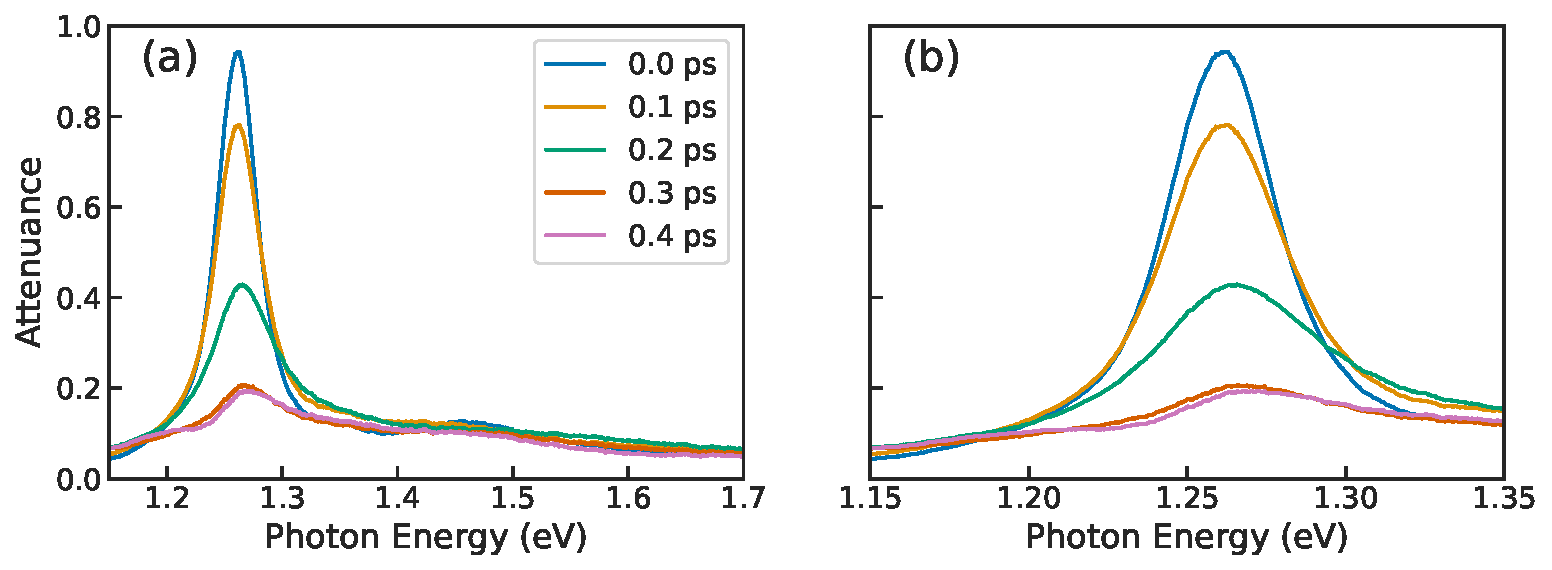
\includegraphics[height=2.4in]{images/chapter_my_data/Weilu_CNT_4mW_E11_decay} \phantomsubcaption}
	{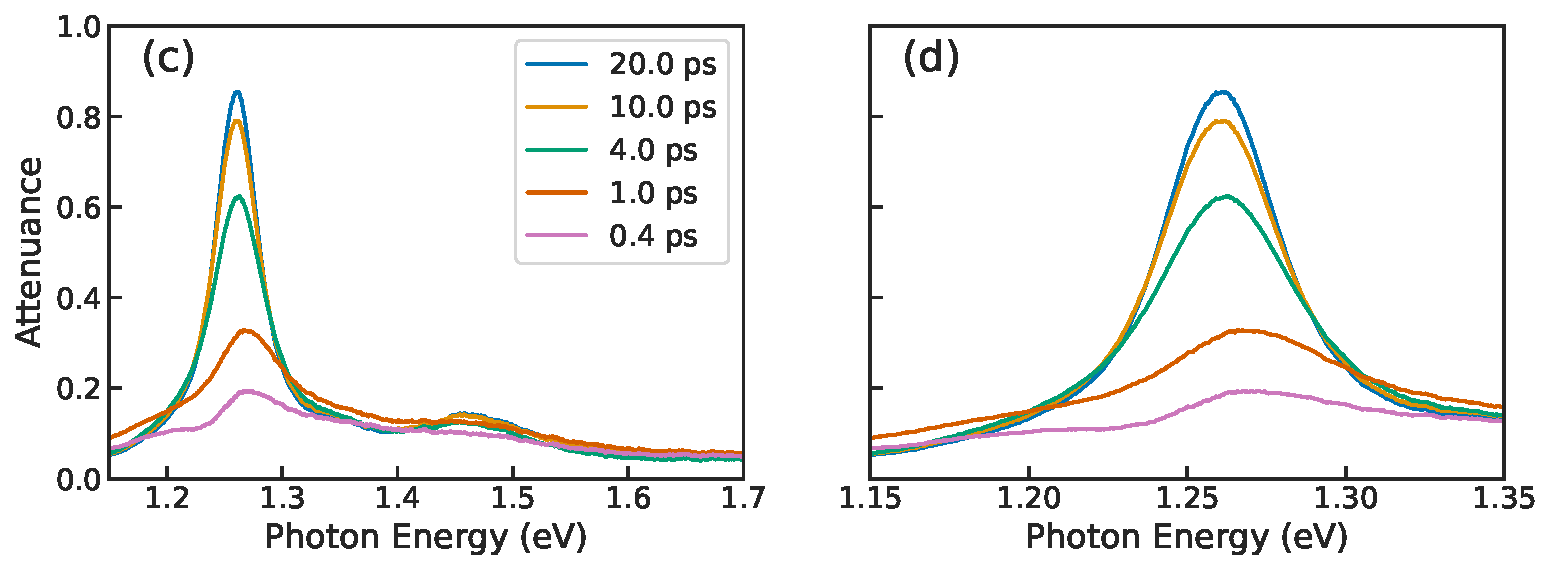
\includegraphics[height=2.4in]{images/chapter_my_data/Weilu_CNT_4mW_E11_recovery} \phantomsubcaption}
	\caption{Attenuance traces measured at the indicated time delay after resonantly exciting the $E_{22}$ transition with a fluence of 7.82 GW/cm$^2$. (a) Total attenuance showing the decay of the absorption at the $E_{11}$ peak at 1.26 eV as well as the attenuation of the phonon sideband located at 1.35 eV. (b) A close-up of the changes $E_{11}$ spectral region shown in Figure (a). (c) Total attenuance at later times showing the recovery of the $E_{11}$ and phonon sideband peaks. (d) A close-up of the changes $E_{11}$ spectral region shown in Figure (c)}
\end{figure}

\begin{figure}[ht]
	\centering
	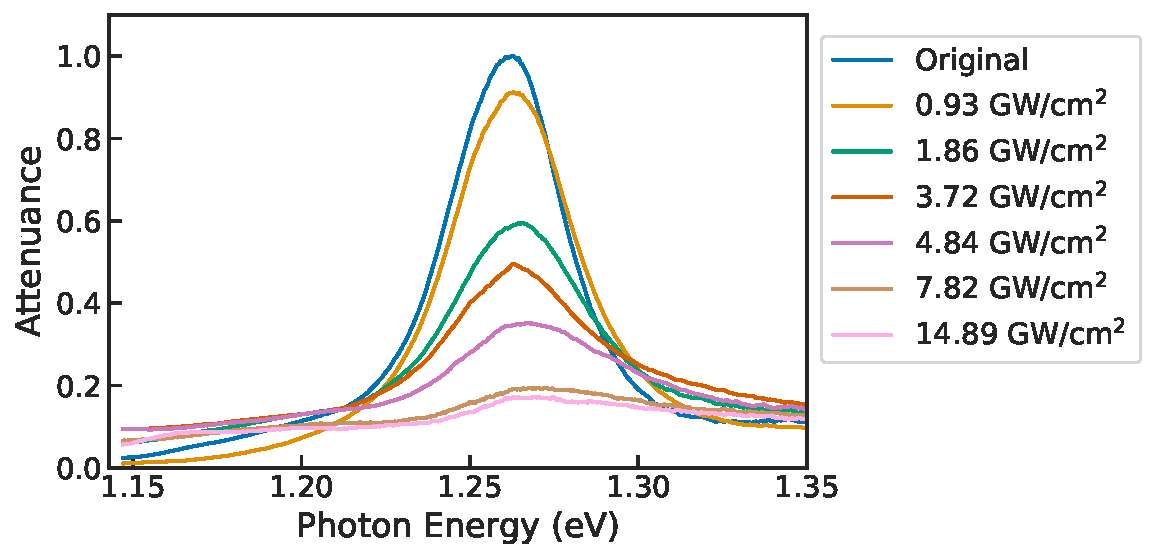
\includegraphics[height=2.4in]{images/chapter_my_data/Weilu_CNT_abs_max_change}
	\caption{{\color{red}UNFINISHED} Maximum decay of the $E_{11}$ peak observed at the labeled excitation power densities. At higher power densities, the $E_{11}$ resonance diminishes more and more due to the creation of carriers. The peak also slightly blueshifts and broadens.}
	\label{fig:weilu_cnt_max_decay}
\end{figure}

\begin{figure}[ht]
	\centering
	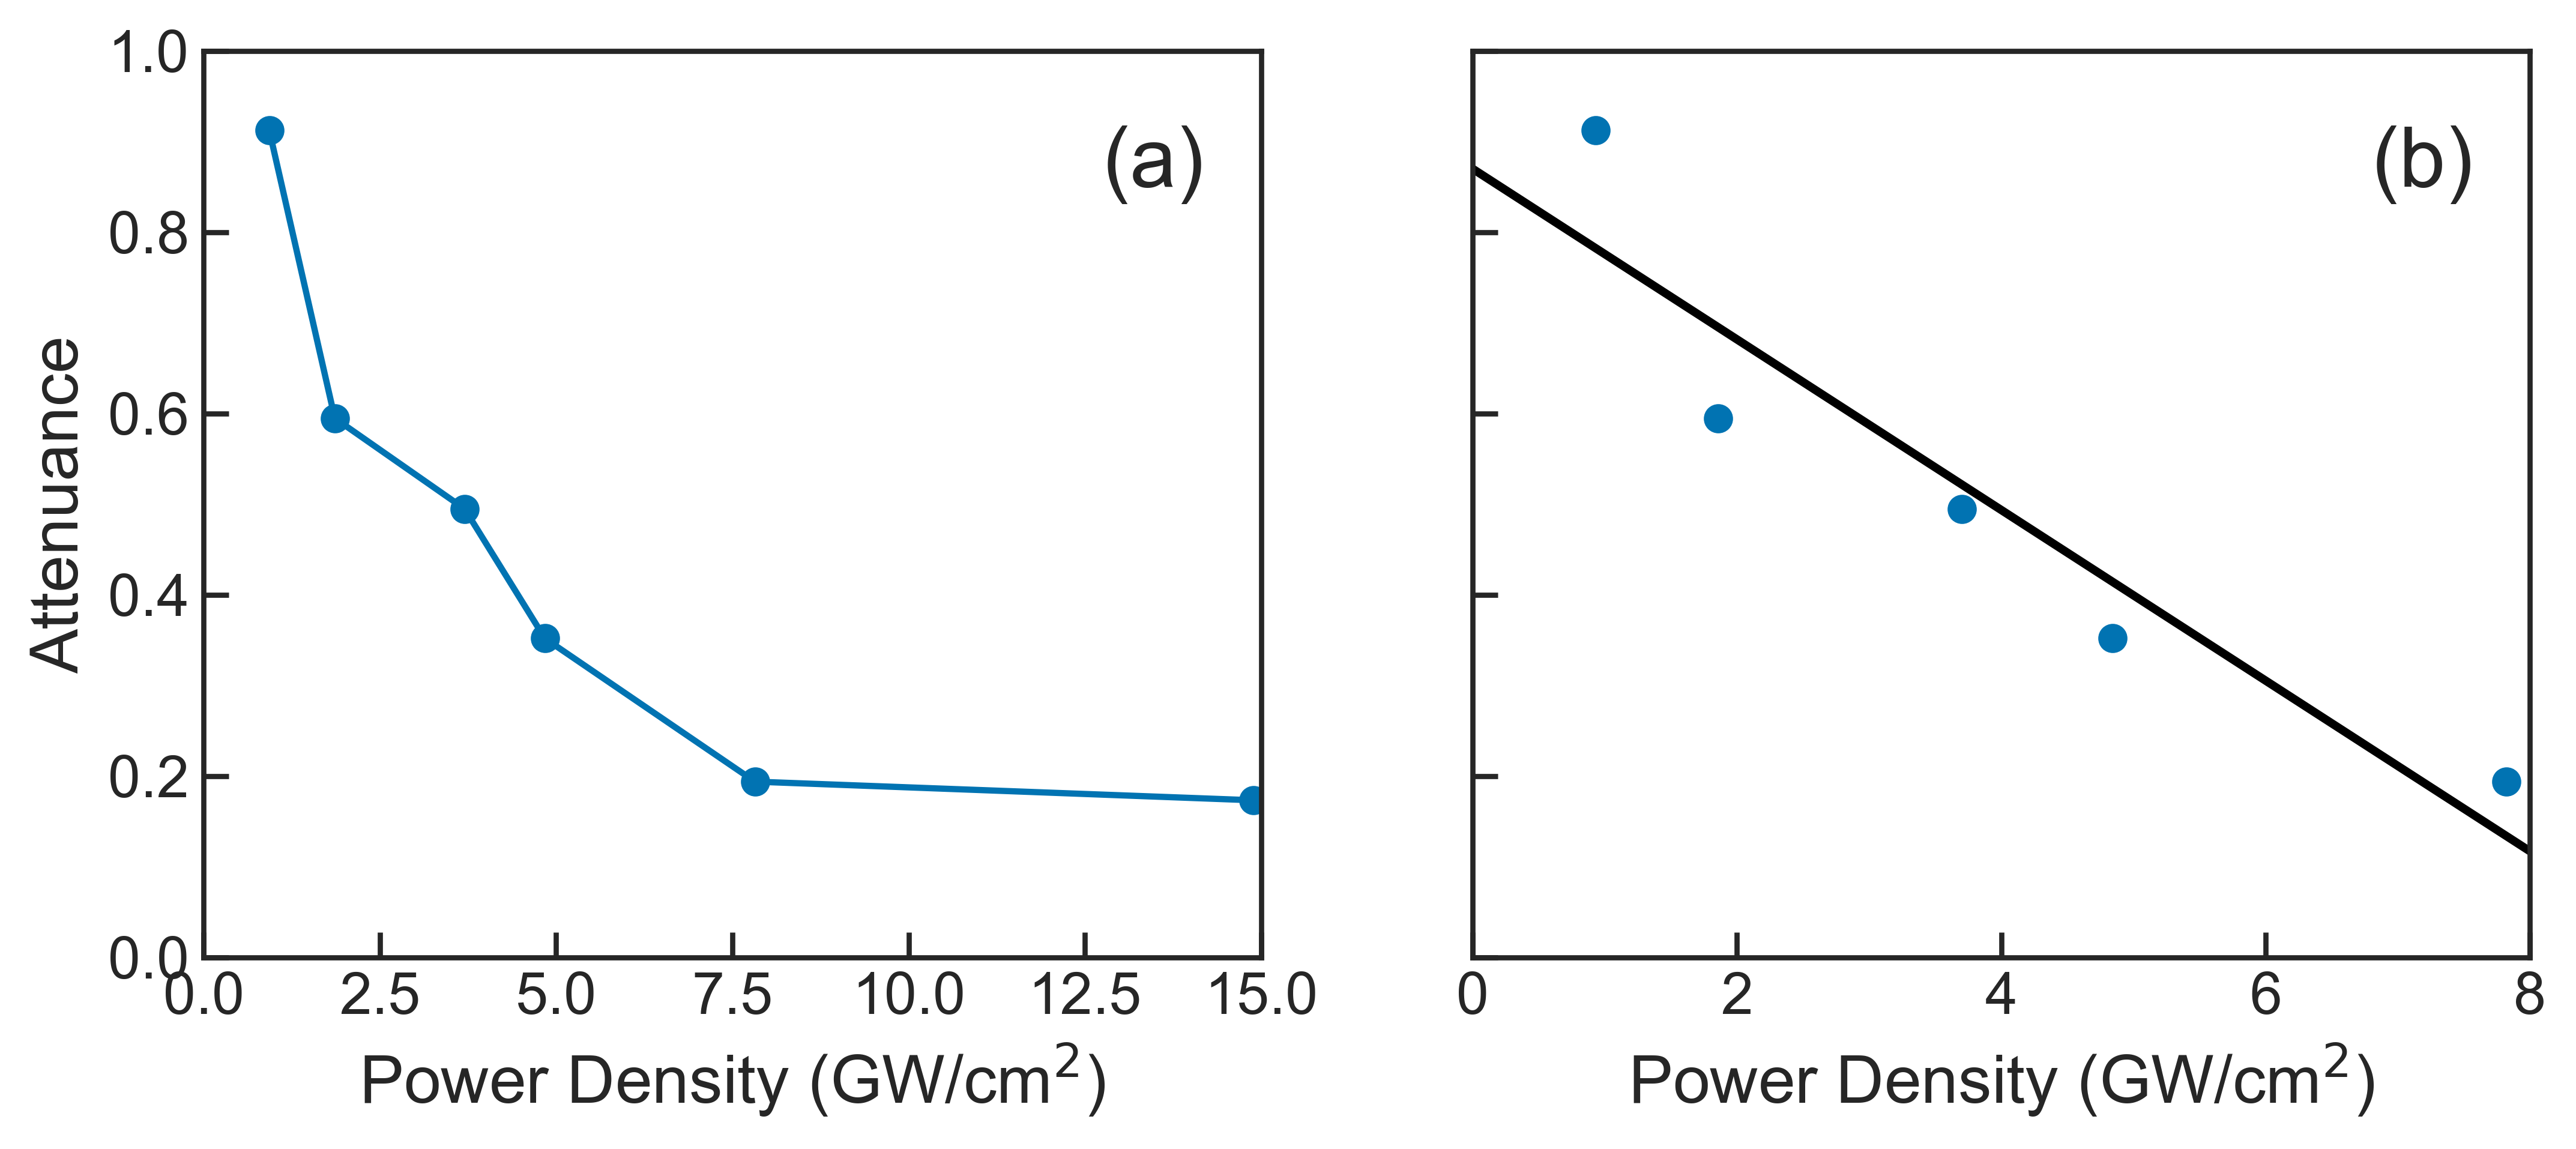
\includegraphics[height=2.4in]{images/chapter_my_data/Weilu_CNT_max_attenuance_and_fit}
	\caption{Maximum attenuance of the $E_{11}$ peak as a function of power density obtained from Figure \ref{fig:weilu_cnt_max_decay}. Photo-bleaching of the $E_{11}$ resonance appears to saturate above a power density of 8 GW/cm$^2$. The right-hand plot shows that below power densities of 8 GW/cm$^2$, the decay of the $E_{11}$ peak is linearly proportional to the power density.}
\end{figure}

\begin{figure}[ht]
	\centering
	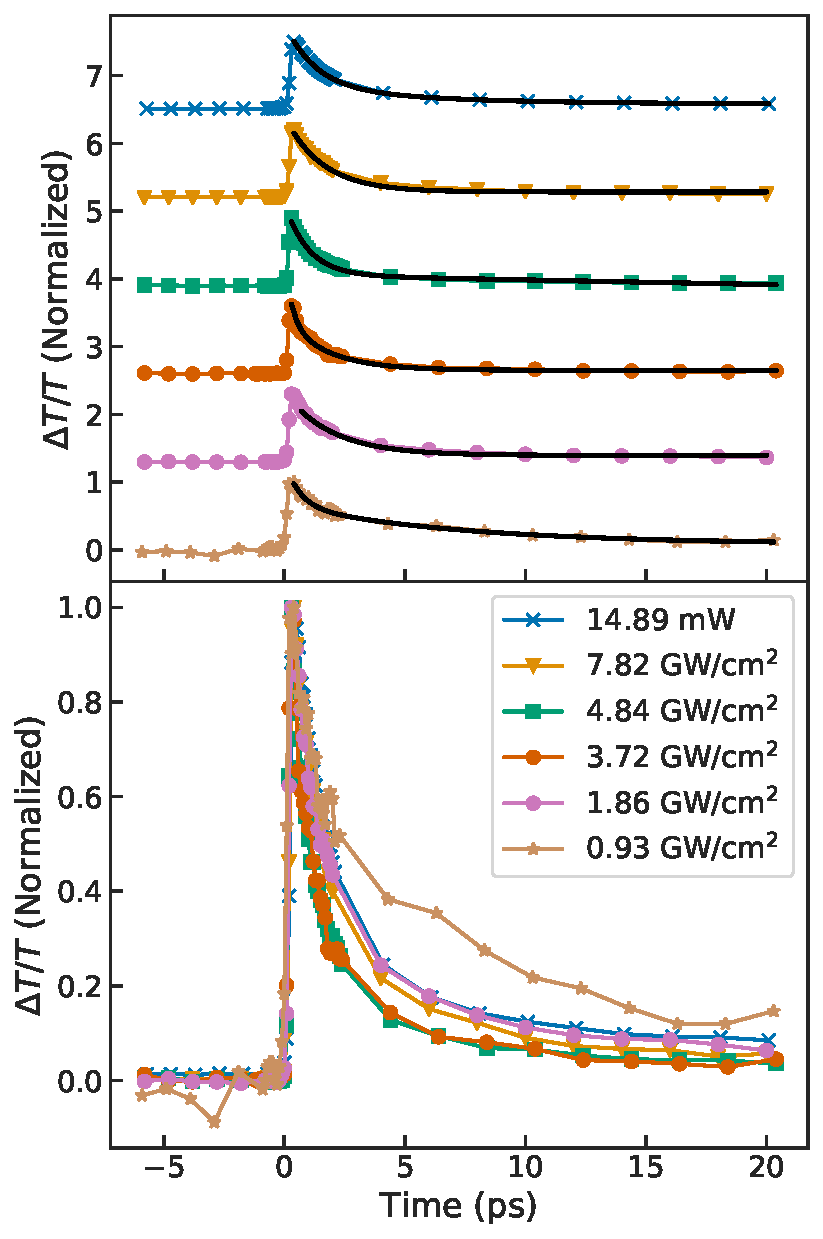
\includegraphics[height=5.4in]{images/chapter_my_data/Weilu_CNT_diff_trans_fits_and_normalized}
	\caption{Data}
\end{figure}




\begin{figure}[ht]
	\centering
	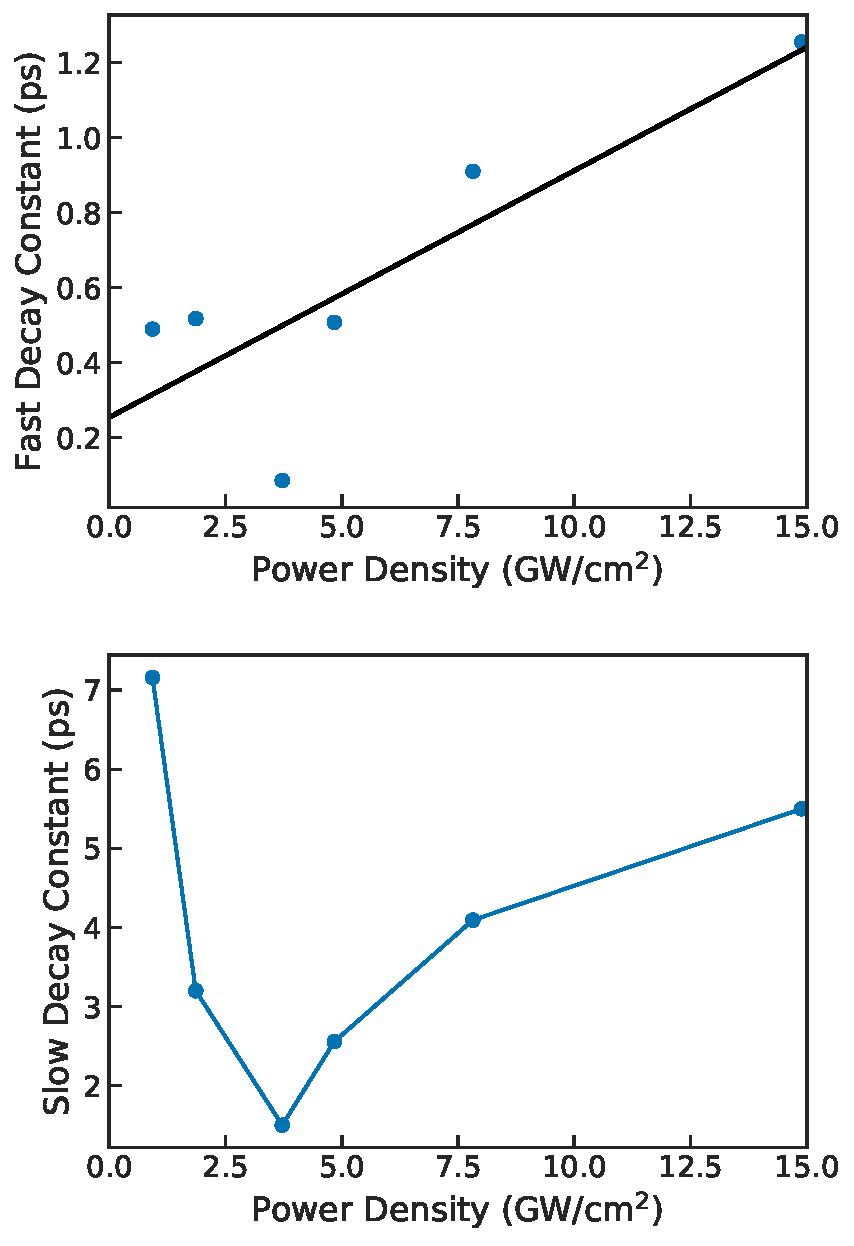
\includegraphics[height=5.4in]{images/chapter_my_data/Weilu_CNT_Fast_Slow_Decay_Const}
	\caption{Data}
\end{figure}


\clearpage
\subsection{PFO-Wrapped (6,5)-Enriched Dispersion}

E11 broadens and blueshifts slightly. In data with better signal-to-noise ratio, also observe absorption bleaching of phonon sideband.

\begin{figure}[ht]%
	\centering
	{\includegraphics[height=2.4in]{images/chapter_my_data/Jan_CNT_ABS_1mW_decay} \phantomsubcaption}
	{\includegraphics[height=2.4in]{images/chapter_my_data/Jan_CNT_ABS_1mW_recovery} \phantomsubcaption}
	\caption{{\color{red} UNFINISHED}}
\end{figure}

\begin{figure}[ht]
	\centering
	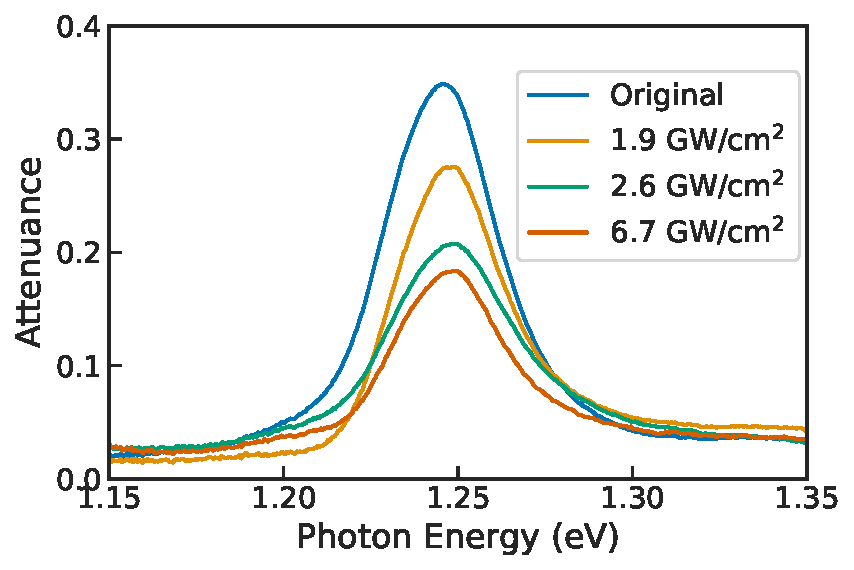
\includegraphics[height=2.4in]{images/chapter_my_data/Jan_CNT_max_abs_change}
	\caption{{\color{red} UNFINISHED}}
\end{figure}

\begin{figure}[ht]
	\centering
	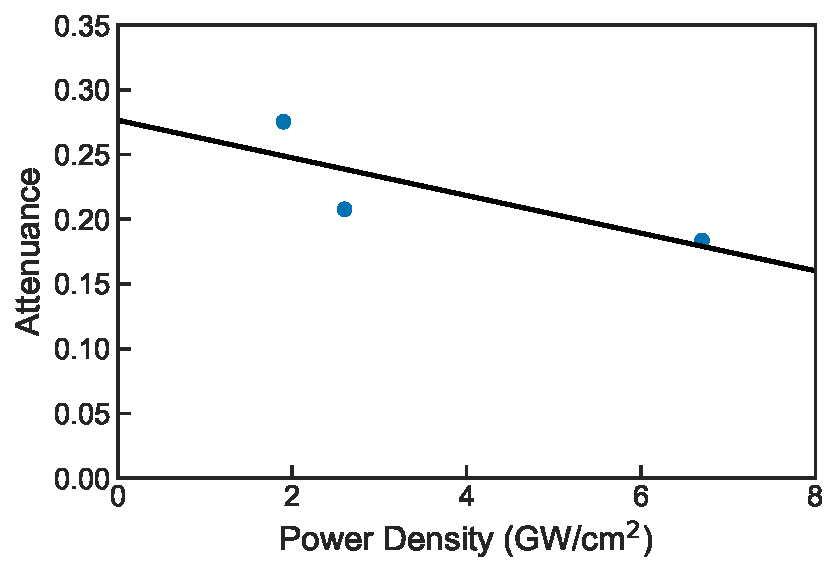
\includegraphics[height=2.4in]{images/chapter_my_data/Jan_CNT_max_attenuance_and_fit}
	\caption{{\color{red} UNFINISHED}}
\end{figure}

\begin{figure}[ht]
	\centering
	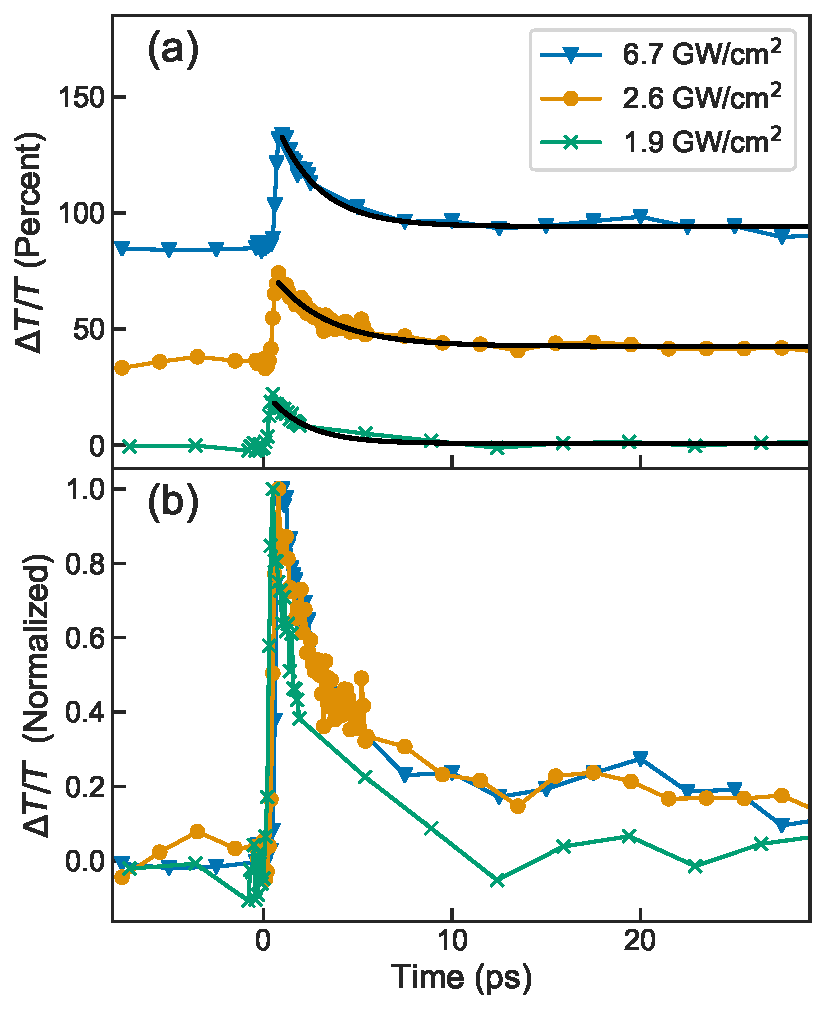
\includegraphics[height=4.4in]{images/chapter_my_data/Jan_CNT_diff_trans_fits_and_normalized}
	\caption{{\color{red} UNFINISHED}}
\end{figure}

\begin{figure}[ht]
	\centering
	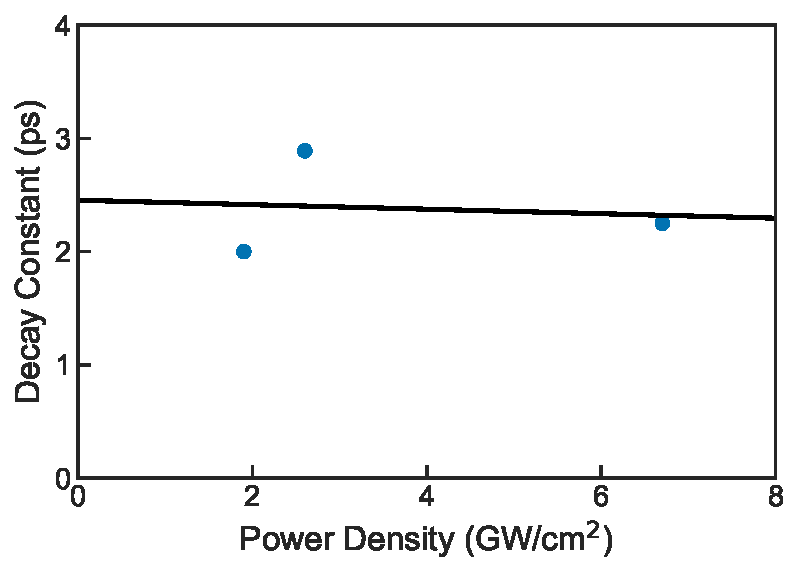
\includegraphics[height=2.4in]{images/chapter_my_data/Jan_CNT_decay_const_fit}
	\caption{{\color{red} UNFINISHED}}
\end{figure}

Data exhibits bi-exponential decay process.


Only probing bright excitons.

\clearpage

\section{Discussion}

Exciton-Exciton annihilation supposedly efficient \cite{murakami2009existence}. If this is the case, E11 should not be absorption bleached.


\section{Conclusions}
